\chapter{UTXO \small{\textsf{DRAFT}}}

\section{Introduction}
Public verifiability of money consists of two parts:
\begin{itemize}
    \item Money creation
    \item Ownership
\end{itemize}
Focus of this lecture: How to verify ownership when money changes hands?
\section{UTXO Model}
We use a graph to represent transactions and the ownership of coins.
Transactions are represented as circles (nodes) with inputs and outputs (edges). Outputs signify receiver(s) of money and inputs signify the sender(s). Both senders and receivers are represented by public keys. An outgoing edge that doesn't connect to a node is referred to as an ``unspent" transaction output (UTXO), and is an element of the UTXO set. A payment from public key $pk_a$ to public key $pk_b$ can be visualised in Figure~\ref{fig:tx_model}.
Note that nodes in this graph are not related to nodes in the network. The senders and receivers of transactions are not necessarily nodes in the network or block miners.

\begin{figure}[h]
\begin{center}
    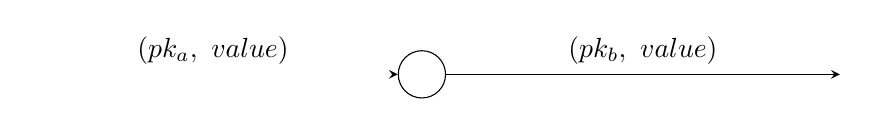
\begin{tikzpicture}

    \node[draw,
        circle,
        minimum size=0.6cm,
        fill=none
    ] (node) at (0,0){};
    \draw[-stealth] -- (-5,0) -- (node.west)
        node[midway,above]{$(pk_a, \ value)$};
    \draw[-stealth] (node.east) -- ++ (5,0)
        node[midway,above]{$(pk_b, \ value)$};

    \end{tikzpicture}
\end{center}
\caption{Representation of a transaction}
\label{fig:tx_model}
\end{figure}


Transactions are connected to one another to form a graph, where the output of a prior transaction becomes the input to a new transaction, as shown in Figure 2. This allows the network to verify that there was a prior transaction that gave money to the sender of a new transaction. For now, we will take money creation for granted and assume that there was an initial transaction that created money and gave it to some public key(s) to start with.
\begin{figure}[h]
\begin{center}
    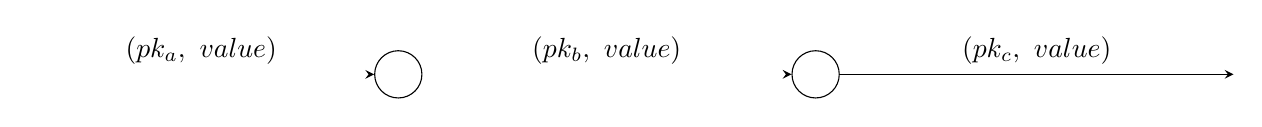
\begin{tikzpicture}

    \node[draw,
        circle,
        minimum size=0.6cm,
        fill=none
    ] (node) at (0,0){};
    \node[draw,
        circle,
        minimum size=0.6cm,
        fill=none
    ] (node1) at (-5.3,0){};
    \draw[-stealth] -- (-10,0) -- (node1.west)
        node[midway,above]{$(pk_a, \ value)$};
    \draw[-stealth] -- (-5,0) -- (node.west)
        node[midway,above]{$(pk_b, \ value)$};
    \draw[-stealth] (node.east) -- ++ (5,0)
        node[midway,above]{$(pk_c, \ value)$};
    \end{tikzpicture}
\end{center}
\caption{The chaining of transactions}
\label{fig:tx_model}
\end{figure}

A chain of transactions is called a ``coin". A coin has a
current owner, denoted in the final outgoing output edge which is not connected to another transaction as input. A coin also has a history of its previous owners. An additional facet of the UTXO model is that all coins are fully spent. In transactions where we don't want to spend the entire coin, we can ``spend" any remainder on ourselves (i.e. keep the change) to maintain the ``fully spent" requirement. These types of transactions will be visualised by a node with two output edges: one edge will have the public key of the recipient of a payment, and the other will have the public key of the payer, as shown in Figure 3. Transactions can also have multiple different inputs (from different or the same public key(s)). For instance, a user could combine two paychecks to purchase a car and receive change by creating a transaction with 2 inputs (each paycheck) and 2 outputs (car dealer and change). This is shown in Figure 4.

\begin{figure}[h]
\begin{center}
    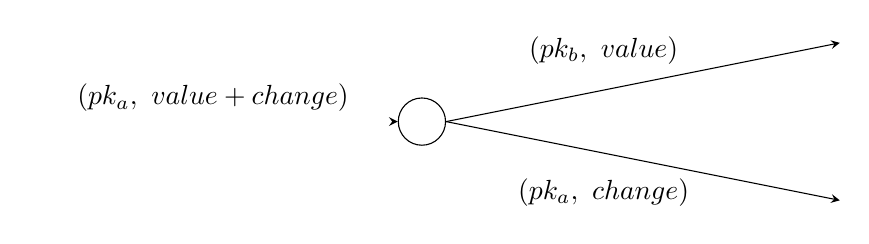
\begin{tikzpicture}

    \node[draw,
        circle,
        minimum size=0.6cm,
        fill=none
    ] (node) at (0,0){};
    \draw[-stealth] -- (-5,0) -- (node.west)
        node[midway,above]{$(pk_a, \ value + change)$};
    \draw[-stealth] (node.east) -- ++ (5,1)
        node[xshift=-3cm, yshift=-0.1cm]{$(pk_b, \ value)$};
    \draw[-stealth] (node.east) -- ++ (5,-1)
        node[xshift=-3cm, yshift=0.1cm]{$(pk_a, \ change)$};

    \end{tikzpicture}
\end{center}
\caption{Representation of a transaction with two outputs}
\label{fig:tx_model}
\end{figure}

\begin{figure}[h]
\begin{center}
    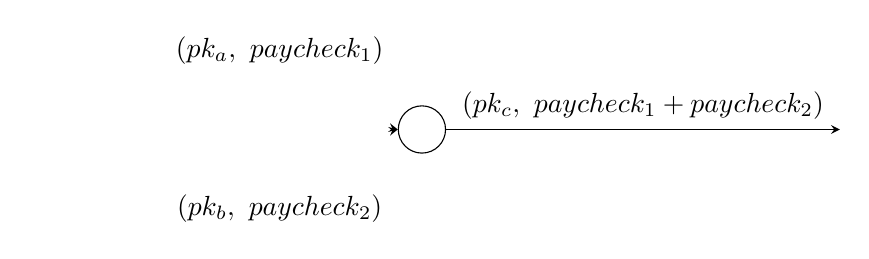
\begin{tikzpicture}

    \node[draw,
        circle,
        minimum size=0.6cm,
        fill=none
    ] (node) at (0,0){};
    \draw[-stealth] -- (-5,1) -- (node.west)
        node[xshift=-1.5cm, yshift=1cm]{$(pk_a, \ paycheck_1)$};
    \draw[-stealth] -- (-5,-1) -- (node.west)
        node[xshift=-1.5cm, yshift=-1cm]{$(pk_b, \ paycheck_2)$};
    \draw[-stealth] (node.east) -- ++ (5,0)
        node[midway,above]{$(pk_c, \ paycheck_1 + paycheck_2)$};

    \end{tikzpicture}
\end{center}
\caption{Representation of a transaction with two inputs}
\label{fig:tx_model}
\end{figure}

The UTXO set (Unspent Transactions Output set) is the set of all unspent transaction outputs. The sum of all values in the UTXO set equals the amount of money in existence. The amount of money owned by a user, e.g. Alice, is the sum of all values in the UTXO for which Alice holds the corresponding secret key ($sk$).

\subsection{Steps for Getting Paid (Strawman Scheme)}
\begin{enumerate}
    \item ($pk$, $sk$) $\leftarrow$ Gen($1^k$) -- Generate public and secret keys.
    \item Send $pk$ to payer (don't need to do this on-chain).
    \item Payer creates a transaction that pays the recipient.
    \item Payer broadcasts this on the network such that all nodes receive the transaction via the gossip protocol.
    \item Validate transaction (check the amount, etc.).
    \item Payment is confirmed.
\end{enumerate}

As an example, consider a situation in which Charlie wants to create a transaction that transfers 1 unit to Alice. Charlie requests Alice for her public key. He will then create a transaction. The transaction includes the amount, Alice's public key ($pk_{A})$, and a pointer to the UTXO that is being spent. The UTXO must be owned by Charlie, i.e. Charlie knows the secret key ($sk_{C}$) corresponding to the public key of the UTXO. Charlie must sign the transaction using his secret key $sk_{C}$ to prove his ownership of the UTXO and so that the transaction cannot be changed. He then broadcasts the transaction to the network and it is validated (by Alice and other nodes).

For Marabu, the unit of money will be called a \emph{bu}. Because computers typically have trouble representing floating point numbers, for Marabu, all transaction amounts will be represented as integer amounts of a unit. This unit will be $10^{-12}$ of a bu (a \emph{picabu}) and all transactions will be represented as number of picabu.
This is similar to Bitcoin where all transaction amounts are represented in number of Satoshis ($1$ Satoshi = $10^{-8}$ bitcoin).

\subsection{Law of Conservation}

The law of conservation requires inputs to strictly equal outputs, while the ``weak" law of conservation requires inputs to exceed or equal outputs (money \emph{can} be destroyed).

\subsection{Format of a transaction}
An outpoint defines a single output of a prior transaction and is represented by the transaction id (the hash of a transaction) and the index (because a transaction may have multiple outputs) of the output of the prior transaction. Transactions are represented as an array of inputs and an array of outputs. Each element of the input array is a tuple of an outpoint and a signature of the transaction under the secret key of the public key associated with that outpoint. Each element in the output array is a tuple of a public key and the value to be given to that public key. A transaction is represented like:

\begin{verbatim}
  tx = {inputs: [{outpoint: {txid, index}, signature}],
        outputs: [{public key, value}]}
 \end{verbatim}

\subsection{Creating a transaction:}
\begin{enumerate}
    \item Create a transaction with the public key of the receiver(s) and the value in the output(s).
    \item Find elements of the UTXO set to constitute the required amount.
    \item Sign the entire transaction with the respective secret keys of all UTXOs being spent. While signing the transaction, the signatures are first replaced by \verb|null| to create an unsigned transaction. The unsigned transaction is used as the message for generating the signatures. Then the signatures are put into the transaction to create a signed transaction.
    \item Broadcast signed transaction.
\end{enumerate}

When transactions are broadcasted, instead of the entire transaction being broadcasted, just the hash of the transaction is broadcasted (in order to reduce network traffic). If when verifying, a node does not have a transaction with a matching hash, they will request the network for the full transaction.

\subsection{Validating a transaction:}
\begin{enumerate}
    \item Check that each input point to an existing UTXO
    \item Check signature(s)
    \item Check weak law of conservation
    \item Erase consumed UTXO(s)
    \item Create new UTXO(s)
\end{enumerate}

Each validating node maintains a UTXO set. Validation is done with respect to that UTXO set. Steps 4 and 5 above describe how this UTXO set is updated and maintained.

In our implementation of the Marabu node, if a transaction is not valid, a node should not gossip it further, so as to prevent spam on the network.
